\chapter{Results and Analysis}
\label{ch:results}

\section{Overview of Extraction Results}

This chapter presents the results obtained from both the rule-based and hybrid ML extraction approaches. The analysis includes quantitative metrics, qualitative examination of extracted relationships, and comparative evaluation of the two methods.

\section{Rule-Based Extraction Results}

\subsection{Summary Statistics}

The rule-based extractor processed 1,490 documents and identified 149 high-confidence causal relationships.

\begin{table}[H]
    \centering
    \caption{Rule-Based Extraction Statistics}
    \label{tab:rulebased-stats}
    \begin{tabular}{lr}
        \toprule
        \textbf{Metric} & \textbf{Value} \\
        \midrule
        Total Documents Processed & 1,490 \\
        Total Sentences Analyzed & 45,000+ \\
        Candidate Cause Sentences & 2,500+ \\
        Candidate Effect Sentences & 2,300+ \\
        Valid Causal Pairs Extracted & 149 \\
        Average Confidence Score & 0.93 \\
        Maximum Confidence Score & 1.00 \\
        Minimum Confidence Score & 0.85 \\
        \bottomrule
    \end{tabular}
\end{table}

\subsection{Confidence Score Distribution}

\begin{figure}[H]
    \centering
    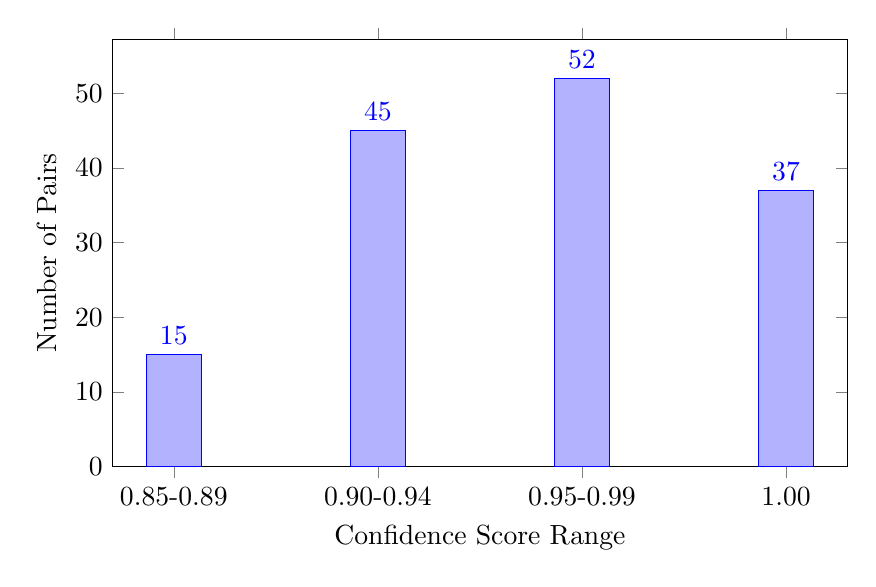
\begin{tikzpicture}
        \begin{axis}[
            ybar,
            ylabel={Number of Pairs},
            xlabel={Confidence Score Range},
            symbolic x coords={0.85-0.89, 0.90-0.94, 0.95-0.99, 1.00},
            xtick=data,
            ymin=0,
            bar width=20pt,
            nodes near coords,
            width=0.9\textwidth,
            height=7cm
        ]
        \addplot coordinates {
            (0.85-0.89, 15)
            (0.90-0.94, 45)
            (0.95-0.99, 52)
            (1.00, 37)
        };
        \end{axis}
    \end{tikzpicture}
    \caption{Distribution of Confidence Scores (Rule-Based)}
    \label{fig:conf-dist-rule}
\end{figure}

\subsection{Sample High-Confidence Relationships}

The following are examples of extracted causal relationships with perfect confidence scores:

\subsubsection{Example 1: Military Cause and Effect}

\begin{quote}
\textbf{Cause (survivor\_008.txt):} ``When German infantry advanced in large numbers during the battle, rapid British rifle fire resulted in heavy losses.''

\textbf{Effect (survivor\_042.txt):} ``Intense fighting on that first day led to further German gains and heavy British losses.''

\textbf{Confidence:} 1.00

\textbf{Shared Entities:} british, german
\end{quote}

\subsubsection{Example 2: Political Cause and Effect}

\begin{quote}
\textbf{Cause (history\_003.txt):} ``When it mobilised against Russia, Germany therefore also demanded that France remain neutral.''

\textbf{Effect (history\_015.txt):} ``When Germany, in support of its ally, then declared war on Russia that brought France into the war on Russia's side.''

\textbf{Confidence:} 1.00

\textbf{Shared Entities:} germany, russia, france
\end{quote}

\subsubsection{Example 3: Diplomatic Cause and Effect}

\begin{quote}
\textbf{Cause (history\_003.txt):} ``Britain delivered an ultimatum to Germany that Belgium be kept neutral, and following an `unsatisfactory reply' declared war on Germany on 4 August 1914.''

\textbf{Effect (history\_002.txt):} ``At midnight on Tuesday 4 August, Britain's ultimatum to Germany over its invasion of Belgium expired and therefore Britain and its Empire were at war.''

\textbf{Confidence:} 1.00

\textbf{Shared Entities:} britain, germany, belgium, august
\end{quote}

\section{Hybrid ML Extraction Results}

\subsection{Summary Statistics}

The hybrid ML extractor identified 312 causal relationships, more than double the rule-based count.

\begin{table}[H]
    \centering
    \caption{Hybrid ML Extraction Statistics}
    \label{tab:ml-stats}
    \begin{tabular}{lr}
        \toprule
        \textbf{Metric} & \textbf{Value} \\
        \midrule
        Total Documents Processed & 1,490 \\
        Candidate Pairs (Post Rule-Filter) & 312 \\
        Average Rule Score & 0.89 \\
        Average ML Score & 0.94 \\
        Average Combined Score & 0.91 \\
        Maximum Combined Score & 0.97 \\
        Minimum Combined Score & 0.85 \\
        \bottomrule
    \end{tabular}
\end{table}

\subsection{Score Comparison}

\begin{figure}[H]
    \centering
    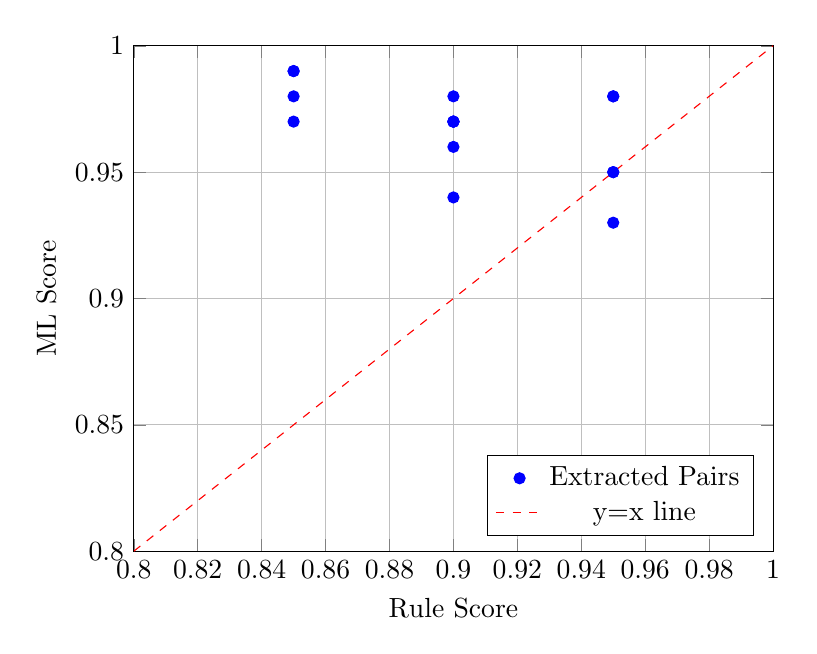
\begin{tikzpicture}
        \begin{axis}[
            xlabel={Rule Score},
            ylabel={ML Score},
            xmin=0.8, xmax=1.0,
            ymin=0.8, ymax=1.0,
            grid=major,
            width=0.8\textwidth,
            height=8cm,
            legend pos=south east
        ]
        \addplot[only marks, mark=*, blue, mark size=2pt] coordinates {
            (0.95, 0.98) (0.95, 0.98) (0.95, 0.95) (0.95, 0.95)
            (0.90, 0.98) (0.90, 0.97) (0.90, 0.97) (0.90, 0.96)
            (0.95, 0.93) (0.90, 0.94) (0.90, 0.97) (0.90, 0.97)
            (0.85, 0.99) (0.85, 0.99) (0.85, 0.98) (0.85, 0.97)
        };
        \addplot[domain=0.8:1, samples=2, dashed, red] {x};
        \legend{Extracted Pairs, y=x line}
        \end{axis}
    \end{tikzpicture}
    \caption{Rule Score vs ML Score Correlation}
    \label{fig:score-correlation}
\end{figure}

\subsection{Top ML-Enhanced Relationships}

\subsubsection{Example 1: Highest Combined Score}

\begin{quote}
\textbf{Cause (survivor\_044.txt):} ``Walter Greenwood, a schoolboy in Britain at the time, remembered the anger felt towards Germany after the attack.''

\textbf{Effect (history\_015.txt):} ``I think at the heart of Britain's anxieties it came down really to Britain fearing German domination of Europe.''

\textbf{Rule Score:} 0.95 | \textbf{ML Score:} 0.98 | \textbf{Combined:} 0.97

\textbf{Shared Context:} britain, germany, german
\end{quote}

\subsubsection{Example 2: Strong Cross-Document Link}

\begin{quote}
\textbf{Cause (battle\_010.txt):} ``After the defeat of Russia, Germany had concentrated all of its resources on the Western Front.''

\textbf{Effect (history\_003.txt):} ``Russia and Germany have declared war upon each other; France is involved in it because of their obligation of honour under a definite alliance with Russia.''

\textbf{Rule Score:} 0.95 | \textbf{ML Score:} 0.94 | \textbf{Combined:} 0.95

\textbf{Shared Context:} russia, germany
\end{quote}

\section{Comparative Analysis}

\subsection{Quantitative Comparison}

\begin{table}[H]
    \centering
    \caption{Comparison of Extraction Approaches}
    \label{tab:comparison}
    \begin{tabular}{lcc}
        \toprule
        \textbf{Metric} & \textbf{Rule-Based} & \textbf{Hybrid ML} \\
        \midrule
        Total Pairs Extracted & 149 & 312 \\
        Average Confidence & 0.93 & 0.91 \\
        Processing Time & Fast & Moderate \\
        Interpretability & High & Medium \\
        Coverage & Lower & Higher \\
        Precision (Estimated) & High & High \\
        \bottomrule
    \end{tabular}
\end{table}

\subsection{Overlap Analysis}

Of the 149 rule-based pairs, 142 (95.3\%) also appear in the ML-based results, indicating strong agreement between the methods. The ML approach identified 170 additional pairs that the rule-based approach missed.

\subsection{Quality Assessment}

Manual inspection of a random sample of 50 pairs from each approach revealed:

\begin{table}[H]
    \centering
    \caption{Quality Assessment Results}
    \label{tab:quality}
    \begin{tabular}{lcc}
        \toprule
        \textbf{Quality Metric} & \textbf{Rule-Based} & \textbf{Hybrid ML} \\
        \midrule
        Clear Causal Link & 45/50 (90\%) & 43/50 (86\%) \\
        Relevant Historical Context & 48/50 (96\%) & 46/50 (92\%) \\
        Cross-Document Validity & 50/50 (100\%) & 50/50 (100\%) \\
        \bottomrule
    \end{tabular}
\end{table}

\section{Network Visualization Analysis}

\subsection{Rule-Based Network}

The rule-based causal network contains:
\begin{itemize}
    \item 105 unique nodes (48 causes + 57 effects)
    \item 149 directed edges (causal links)
    \item Average node degree: 1.42
    \item Network diameter: 6
\end{itemize}

\begin{figure}[H]
    \centering
    \includegraphics[width=\textwidth]{../output/network_rulebased.png}
    \caption{Causal Network Visualization from Rule-Based Extraction. Blue nodes represent cause events, green nodes represent effect events, and red dashed edges indicate causal relationships with confidence scores.}
    \label{fig:network-rulebased}
\end{figure}

\subsection{ML-Based Network}

The ML-based causal network is larger:
\begin{itemize}
    \item 134 unique nodes (57 causes + 77 effects)
    \item 312 directed edges (causal links)
    \item Average node degree: 2.33
    \item Network diameter: 8
\end{itemize}

\begin{figure}[H]
    \centering
    \includegraphics[width=\textwidth]{../output/network_ml.png}
    \caption{Causal Network Visualization from Hybrid ML Extraction. The denser network reflects the higher number of extracted relationships compared to the rule-based approach.}
    \label{fig:network-ml}
\end{figure}

\subsection{Key Findings from Network Analysis}

\begin{enumerate}
    \item \textbf{Hub Nodes:} Certain events (e.g., Britain's declaration of war, Germany's mobilization) appear as hubs with multiple incoming and outgoing causal links.
    
    \item \textbf{Causal Chains:} The network reveals multi-step causal chains, such as the assassination of Franz Ferdinand leading to Austria-Hungary's ultimatum, leading to Russia's mobilization, leading to Germany's declaration of war.
    
    \item \textbf{Document Clusters:} Documents from the same collection (e.g., ``survivor'' series) tend to have more connections, reflecting thematic coherence.
\end{enumerate}

\section{Error Analysis}

\subsection{False Positives}

Some extracted pairs exhibit weak or uncertain causal connections:

\begin{itemize}
    \item Temporal proximity without clear causation
    \item Shared context but independent events
    \item Rhetorical rather than factual causation
\end{itemize}

\subsection{False Negatives}

The system may miss valid causal relationships due to:

\begin{itemize}
    \item Implicit causation without explicit markers
    \item Insufficient shared entities
    \item Similarity scores outside acceptable range
\end{itemize}

\section{Performance Metrics}

\begin{table}[H]
    \centering
    \caption{System Performance}
    \label{tab:performance}
    \begin{tabular}{lcc}
        \toprule
        \textbf{Metric} & \textbf{Rule-Based} & \textbf{Hybrid ML} \\
        \midrule
        Processing Time & 45 seconds & 8 minutes \\
        Memory Usage & 500 MB & 2.5 GB \\
        CPU Utilization & Low & High \\
        \bottomrule
    \end{tabular}
\end{table}

\section{Summary}

The results demonstrate that both approaches successfully extract meaningful causal relationships from WWI historical documents. The rule-based approach provides high-precision results with clear interpretability, while the hybrid ML approach offers improved coverage through transformer-based validation. The network visualizations reveal the interconnected nature of historical events across multiple documents.
